\documentclass[a4paper,12pt]{article} % тип документа

% report, book

% Рисунки
\usepackage{graphicx}
\usepackage{wrapfig}
\usepackage{mathtext}
\usepackage[left=2cm,right=2cm,
    top=2cm,bottom=2cm,bindingoffset=0cm]{geometry}

\usepackage{hyperref}
\usepackage[rgb]{xcolor}
\hypersetup{				% Гиперссылки
    colorlinks=true,       	% false: ссылки в рамках
	urlcolor=blue          % на URL
}

%  Русский язык

\usepackage[T2A]{fontenc}			% кодировка
\usepackage[utf8]{inputenc}			% кодировка исходного текста
\usepackage[english,russian]{babel}	% локализация и переносы


% Математика
\usepackage{amsmath,amsfonts,amssymb,amsthm,mathtools} 


\usepackage{wasysym}

\author{Артемов Иван, Лежнев Дмитрий Б02-205}
\title{2.2.3 Измерение теплопроводности воздуха при атмосферном давлении}
\date{\today}
\begin{document}
\maketitle

\textbf{Цель работы:} определение коэффициента теплопроводности воздуха при атмосферном давлении и разных температурах по теплоотдаче нагреваемой током нити в цилиндрическом сосуде.

\textbf{Оборудование:} прибор для опредления теплопроводности газов; форвакуумный насос; газгольдер с газом; манометр; магазин сопротивлений; эталонное сопротивление 10 Ом; цифровой вольтметр B7-78/1; источник питания.


\section*{1. Теоретическая часть}

	Основной характеристикой теплопроводности служит коэффициент $\kappa$, являющийся коэффициентом пропорциональности между плотностью потока тепла $q$ и градиентом температуры $dT/dr$ в направлении распространения этого потока
\begin{equation}
	q = -\kappa \frac{dT}{dr}.
\end{equation}

	В цилиндрически симметричной установке, в которой тепловой поток направлен к стенкам цилиндра от нити, полынй поток тепла $Q = qS$ через каждую цилиндрическую поверхность радиуса $r$ должен в стационарном состоянии быть неизменен (как в пространстве, так и во времени). Тогда
\begin{equation}
	Q = -2\pi rL\kappa \frac{dT}{dr} = const,	
\end{equation}
откуда получаем формулу
\begin{equation}
	\label{formula}
	T_1 - T_2 = \frac{Q}{2\pi L\kappa} \ln \frac{r_2}{r_1}.
\end{equation}
Здесь $r_1$ и $T_1$ -- радиус и температура нити, $r_2$ и $T_2$ -- радиус и температура цилиндра.


\section*{2. Экспериментальная установка}

	Схема установки изображена на рис.~\ref{ris:ustanovka}. Тонкая молибденовая нить натянута по оси длинной вертикально стоящей медной трубки\footnote{В нашей установке диаметр проволоки $2r_1 \approx 0,055$ мм, внутренний диаметр трубки $2r_2 \approx 10$ мм, длина $L \approx 355$ мм.}.
	Через штуцер трубка заполняется исследуемым газом. Нить нагревается электрическим током, а её температура $T_1$ определяется по изменению электрического сопротивления. Трубка находится в кожухе, через которой пропускается вода из термостата. Температура воды $T_2$ измеряется термометром, помещенным в термостат. Количество теплоты, протекающей через газ, равно, если принебречь утечками тепла через торцы, количеству теплоты, выделяемому током в нити, и может быть найдено по закону Джоуля-Ленца\footnote{Мощность электрического тока, протекающего через нить: $Q = I^2 R$}. При этом ток в нити определяется по напряжению на включенном последовательно с ней эталонном сопротивлении $R_0 = (10,00 \pm 0,01)$ Ом.
	
	Электрическая часть схемы состоит из источника питания и подключенных к нему последовательно соединенных нити, эталонного сопротивления и магазина сопротивлений $R$, служащего для точной установки тока через нить. Цифровой вольтметр может подключаться как к нити, так и к эталонному сопротивлению, измеряя таким образом напряжение на нити и ток через неё.
	
\begin{figure}[h]
	\center{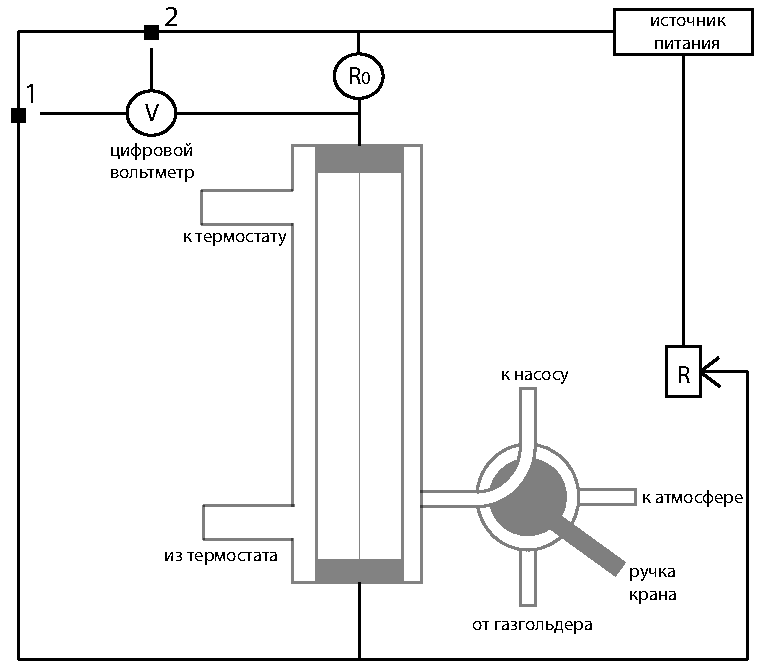
\includegraphics[scale=1]{Draw_1.pdf}}
	\caption{Схема установки для определения теплопроводности газов}
	\label{ris:ustanovka}
\end{figure}



\section*{3. Измерения и обработка данных}
\begin{itemize}
\item[\textbf{1. }]Построим графики зависимости R(P) для температур $24.0^{\circ} C$, \; $29.8^{\circ} C$, \; $45.1^{\circ} C$, \; $65.1^{\circ} C$, \; $80.1^{\circ} C$. Результаты - на рис. 4,5,6,7,8.
\item[\textbf{2. }] Найдя значение $R_0$ для каждого из графиков по МНК, построим график зависимости $R_0(t)$ (рис. 9). Обработав его по МНК, найдём коэффициент $dR/dT$ для нити:
\[\frac{dR}{dT} = (0.0712 \pm 0.0004) \frac{\text{Ом}}{\text{К}} \]
\item[\textbf{3. }] Вычислим значение коэффициента теплопроводности при каждой температуре по формуле:
\begin{equation}\label{formula}
\kappa = \frac{dR/dT}{dR/dQ}  \frac{1}{2\pi L} \ln{\left(\frac{r_2}{r_1}\right)}
\end{equation}

Результаты - в табл. 1.
\item[\textbf{4. }] Построим график зависимости $\kappa(t)$ и $\ln{\kappa} (\ln{t})$ (рис. 8, 9). Предполагая, что $\kappa \sim T^{\beta}$ получим из второго графика:
\[\beta = 0.93 \pm 0.02 \]
Результат отличается от теории ($\kappa \sim \sqrt{T}$) на 86 \%. Этому есть несколько причин. Во-первых, число экспериментальных точек слишком мало, а интервал между ними слишком велик. Во-вторых, формула \eqref{formula} была выведена в предположении, что $\kappa$ не зависит от температуры нити, то есть $\Delta T \ll T$, что тоже не может выполняться с высокой точностью при сильном нагреве нити. И также при выводе формулы \eqref{formula} не были учтены потери через основания цилиндра.
\end{itemize}

	
\noindent


\begin{figure}
\begin{minipage}{\linewidth}
\centering
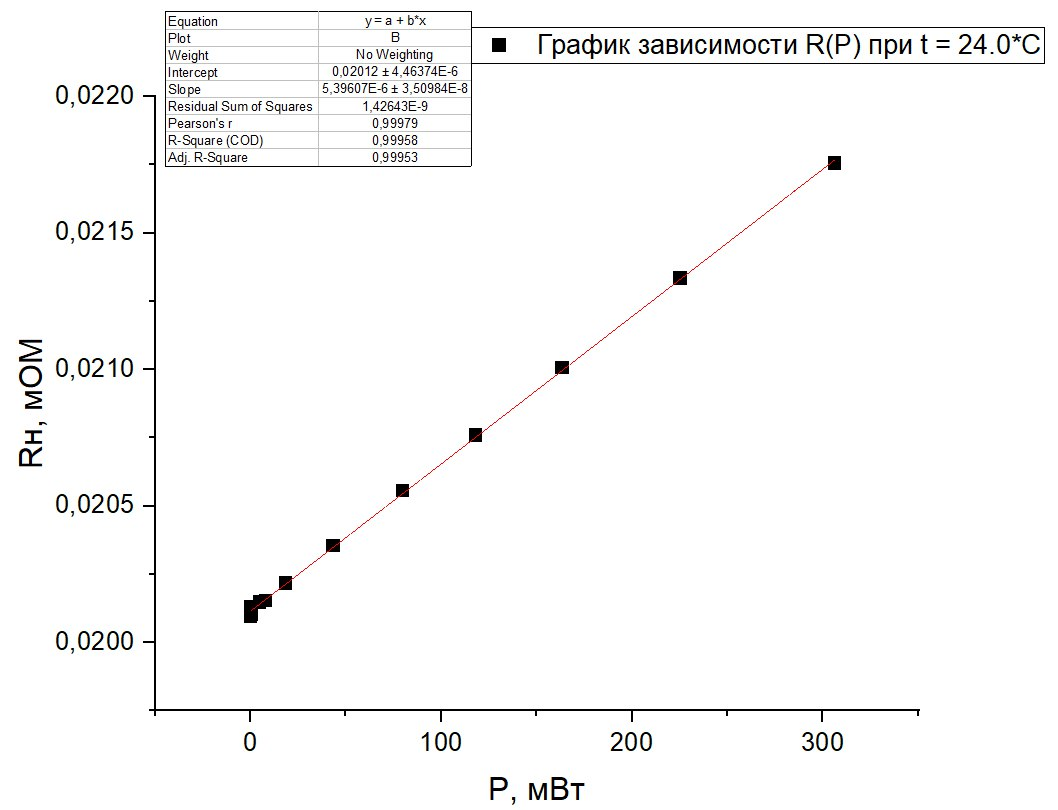
\includegraphics[scale=0.35]{24.0.jpg}
\caption{}
\end{minipage}
\begin{minipage}{\linewidth}
\centering
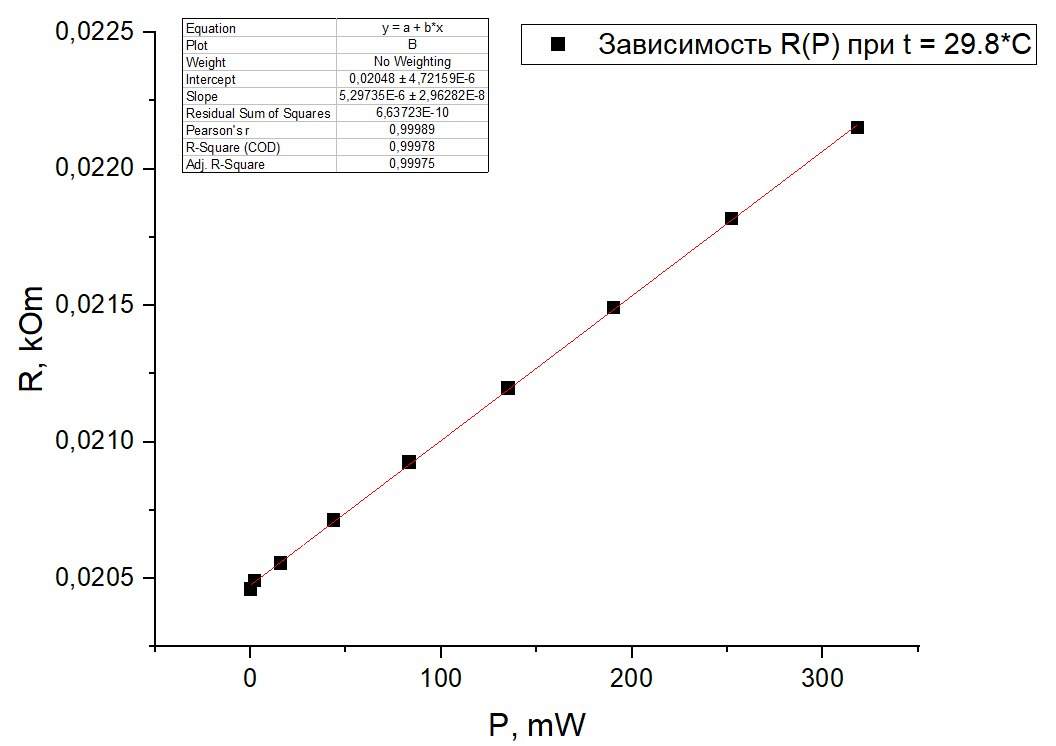
\includegraphics[scale=0.35]{29.8.jpg}
\caption{}
\end{minipage}
\end{figure}

\begin{figure}
\begin{minipage}{\linewidth}
\centering
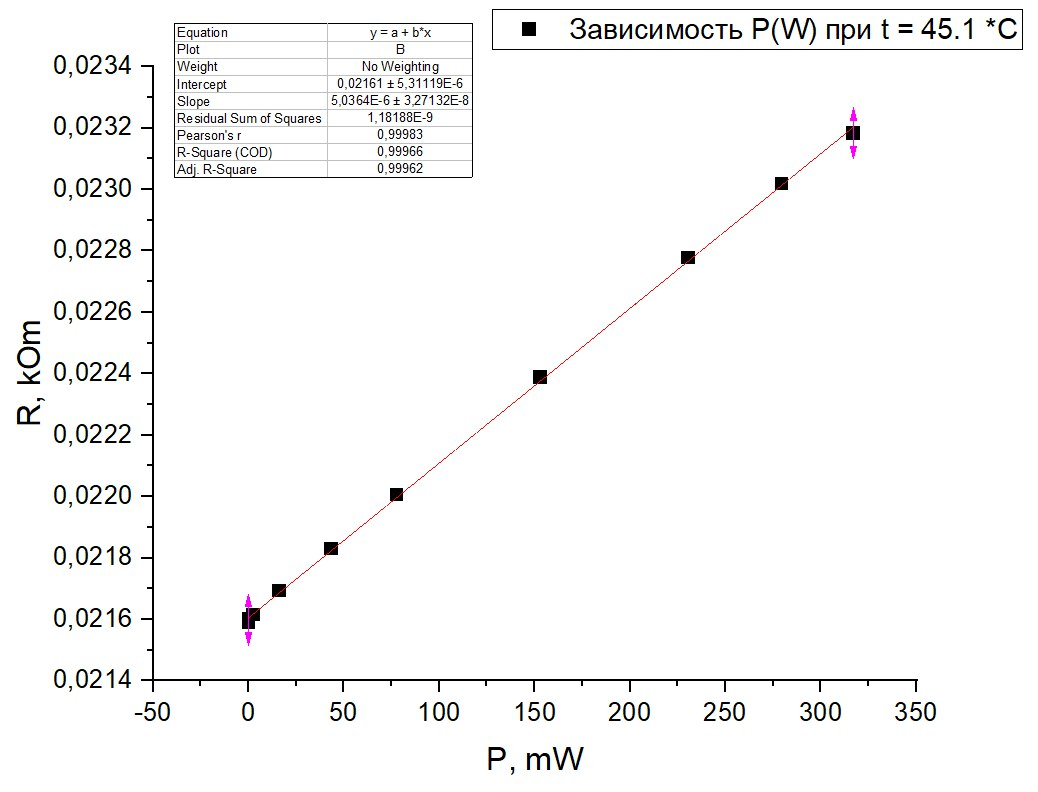
\includegraphics[scale=0.35]{45.1.jpg}
\caption{}
\end{minipage}
\begin{minipage}{\linewidth}
\centering
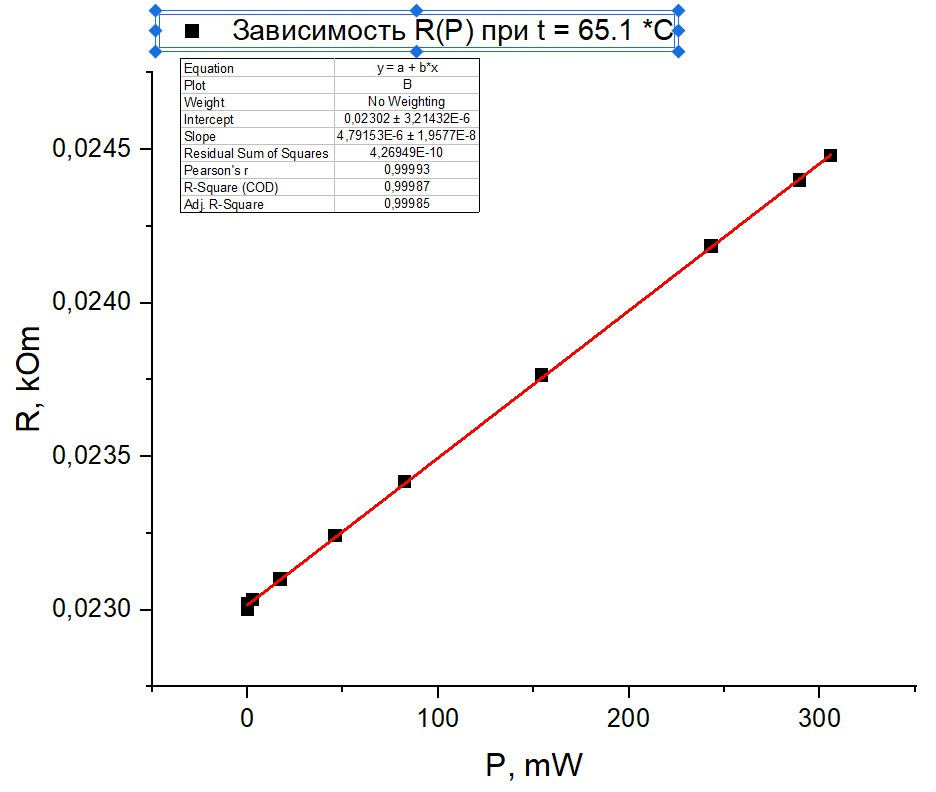
\includegraphics[scale=0.35]{65.1.jpg}
\caption{}
\end{minipage}
\end{figure}

\begin{figure}
\begin{minipage}{\linewidth}
\centering
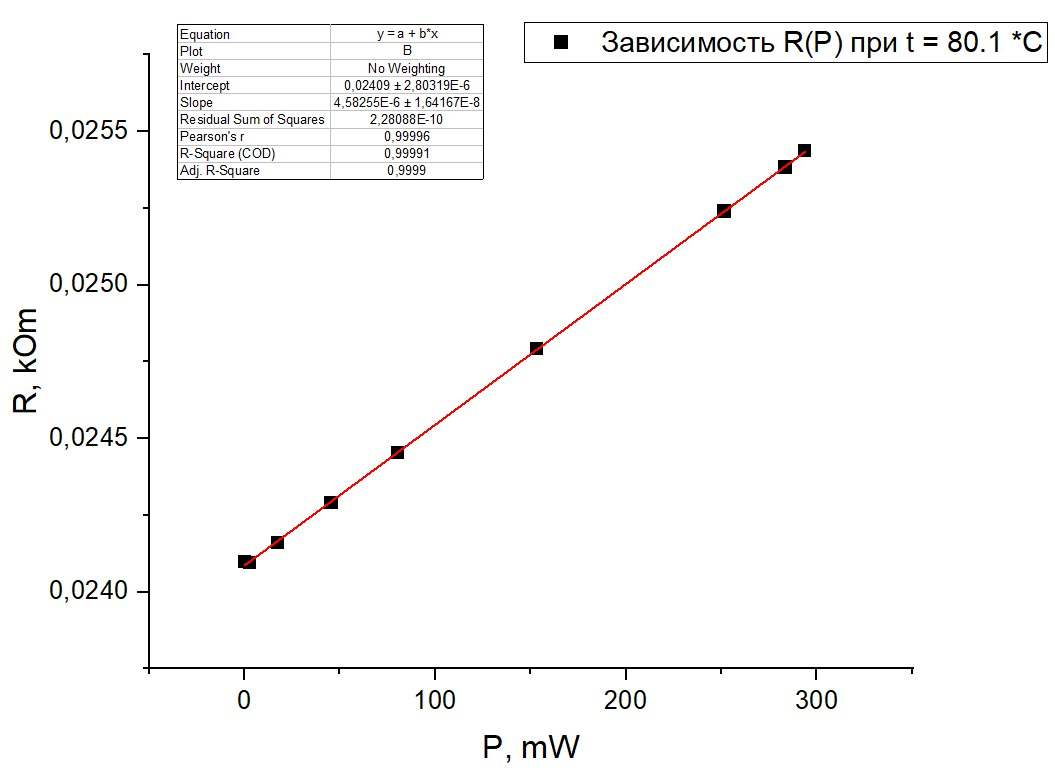
\includegraphics[scale=0.35]{80.1.jpg}
\caption{}
\end{minipage}
\begin{minipage}{\linewidth}
\centering
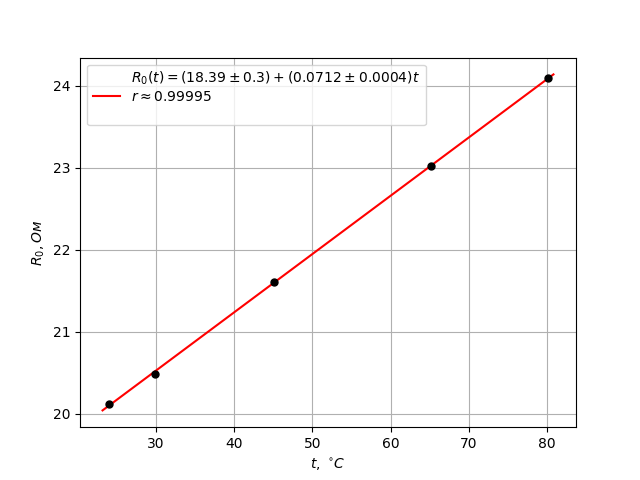
\includegraphics[scale=1]{R0t.png}
\caption{}
\end{minipage}
\end{figure}

\begin{figure}
\begin{minipage}{\linewidth}
\centering
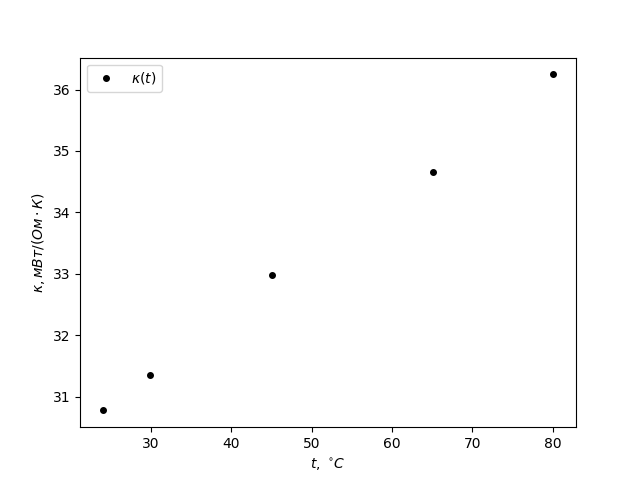
\includegraphics[scale=1]{kappat.png}
\caption{}
\end{minipage}
\begin{minipage}{\linewidth}
\centering
\includegraphics[scale=1]{lnklnt.png}
\caption{}
\end{minipage}
\end{figure}
	
	
\begin{table}[]
\begin{minipage}{\linewidth}
\centering
\begin{tabular}{|c|c|}
\hline
$t, \ ^{\circ}C$ & $\kappa, \text{мВт}/(\text{Ом} \cdot   \text{К})$ \\ \hline
24.0             & $30.8 \pm 0.3$                     \\ \hline
29.8             & $31.4 \pm 0.3$                       \\ \hline
45.1             & $33.0 \pm 0.3$                      \\ \hline
65.1             & $34.0 \pm 0.2$                       \\ \hline
80.1             & $36.3 \pm 0.2$                       \\ \hline
\end{tabular}
\caption{}
\end{minipage}
\end{table}


\section*{4. Вывод}



\begin{enumerate}
\item
	Определили коэффициент теплопроводности воздуха при атмосферном давлении и разных температурах по теплоотдаче нагреваемой током нити в цилиндрическому сосуде. Например при комнатной температуре $t = 24.0 \ ^{\circ} C$, $\kappa = (30.9 \pm 0.3) \text{мВт}/(\text{м} \cdot \text{К})$
	
\item
	В предположении, что $\varkappa = AT^\beta$, рассчитали коэффициент $\beta = 0.93 \pm 0.02$.

\end{enumerate}
\end{document}

\end{document}